\documentclass[a4paper, 11pt, pdftex]{report}
\usepackage{graphicx}
\usepackage{amsmath, amsthm}
\usepackage[T1]{fontenc}
\usepackage[full]{textcomp}
\usepackage[charter]{mathdesign}
\usepackage[utf8]{inputenc}
\usepackage[english]{babel}
%\usepackage[]{showkeys}
\usepackage{hyperref}
\usepackage[all]{hypcap}
\usepackage[noend]{algorithm, algpseudocode}
\usepackage{listingsutf8}
\usepackage{mathtools}
\usepackage[svgnames]{xcolor}
\usepackage{multirow}
\usepackage{enumitem}
\usepackage{caption} 

\usepackage{fullpage}
\setlength\parindent{0pt}
\setlength\parskip{\baselineskip}
\setlength{\abovedisplayskip}{0pt}
\sloppy
\pagestyle{plain}

\usepackage{epigraph}
\setlength\epigraphwidth{.65\textwidth}

\theoremstyle{plain}
\newtheorem{theorem}{Theorem}[chapter]
\newtheorem*{theorem*}{Theorem}

\theoremstyle{definition}
\newtheorem{algo}[theorem]{Algorithm}

\usepackage{chngcntr}
\counterwithin{figure}{chapter}
\counterwithin{table}{chapter}

\makeatletter
\renewcommand*{\thetable}{\arabic{chapter}.\arabic{table}}
\renewcommand*{\thefigure}{\arabic{chapter}.\arabic{figure}}
\let\c@table\c@figure
\makeatother 

\newcommand\T{\rule{0pt}{2.6ex}}
\newcommand\B{\rule[-1.4ex]{0pt}{0pt}} 

\DeclareMathOperator{\ord}{ord}

\begin{document}

\begin{titlepage}
	\centering
	\vspace*{2cm}
	{\scshape\Huge f\textsubscript{12}ecm\par}
	\vspace{2cm}
	{\scshape\Large A program for finding\\the factors of\\the twelfth Fermat number\par}
	\vspace{4cm}
	{\huge\bfseries Elliptic Curve Method\\and\\Probabilities\par}
	\vspace{4cm}
	{\Large\itshape Yves Gallot\par}
	\vfill
	{\large \today\par}
\end{titlepage}

\vspace*{2cm}
{\scshape f\textsubscript{12}ecm} is free source code, under the MIT license.

Copyright (c) 2021, Yves Gallot

Permission is hereby granted, free of charge, to any person obtaining a copy
of this software and associated documentation files (the "Software"), to deal
in the Software without restriction, including without limitation the rights
to use, copy, modify, merge, publish, distribute, sublicense, and/or sell
copies of the Software, and to permit persons to whom the Software is
furnished to do so, subject to the following conditions:

The above copyright notice and this permission notice shall be included in
all copies or substantial portions of the Software.

THE SOFTWARE IS PROVIDED "AS IS", WITHOUT WARRANTY OF ANY KIND, EXPRESS OR
IMPLIED, INCLUDING BUT NOT LIMITED TO THE WARRANTIES OF MERCHANTABILITY,
FITNESS FOR A PARTICULAR PURPOSE AND NONINFRINGEMENT. IN NO EVENT SHALL THE
AUTHORS OR COPYRIGHT HOLDERS BE LIABLE FOR ANY CLAIM, DAMAGES OR OTHER
LIABILITY, WHETHER IN AN ACTION OF CONTRACT, TORT OR OTHERWISE, ARISING FROM,
OUT OF OR IN CONNECTION WITH THE SOFTWARE OR THE USE OR OTHER DEALINGS IN
THE SOFTWARE.


\chapter{Fermat numbers}

\epigraph{Si je puis une fois tenir la raison fondamentale que 3, 5, 17, etc. sont nombres premiers,
il me semble que je trouverai de très belles choses en cette matière,}
{\textit{Fermat à Mersenne \\ 25 décembre 1640}}

Pierre de Fermat conjectured that every number of the form $F_{n} = 2^{2^n} + 1,$ where $n$ is a non-negative integer, is prime \cite{Fermat1}. Today these positive integers are named Fermat numbers. The first five Fermat numbers are prime, but Leonhard Euler proved in 1732 that $641$ divides $F_5$.

$F_6$ was completely factored by T~Clausen, F.~Landry and H.~Le~Lasseur in 1855. In 1970, M.~A.~Morrison and J.~Brillhart cracked $F_7$ by the Continued Fraction method \cite{MorrisonBrillhart1}. In 1980, 		R.~P.~Brent and J.~M.~Pollard used a modification of Pollard's rho method to factor $F_8$. R.~P.~Brent completely factored $F_{11}$ in 1988 by ECM \cite{Brent2}. In 1990, A.~K.~Lenstra, H.~W.~Lenstra, M.~S.~Manasse and J.~M.~Pollard organized a distributed computation on approximately 700 workstations around the world and factored $F_9$ by the Number Field Sieve \cite{Lenstra2ManassePollard}. Finally R.~P.~Brent completely factored $F_{10}$ in 1995 by ECM \cite{Brent2}.

The smallest Fermat number which is not completely factored is $F_{12}$. Six prime factors are known, the 54-digit factor was found by Michael Vang in 2010 using GMP--ECM \cite{Vang1}.

\begin{tabular}{lcl}
	\T $F_5$ &= &$641 \:\cdot\: 6700417$\\
	\T $F_6$ &= &$274177 \:\cdot\: 67280421310721$\\
	\T $F_7$ &= &$59649589127497217 \:\cdot\: 5704689200685129054721$\\
	\T $F_8$ &= &$1238926361552897 \:\cdot\: P_{62}$\\
	\T $F_9$ &= &$2424833 \:\cdot\: 7455602825647884208337395736200454918783366342657 \:\cdot\: P_{99}$\\
	\T $F_{10}$ &= &$45592577 \:\cdot\: 6487031809 \:\cdot\: 4659775785220018543264560743076778192897 \:\cdot\: P_{252}$\\
	\T $F_{11}$ &= &$319489 \:\cdot\: 974849 \:\cdot\: 167988556341760475137 \:\cdot\: 3560841906445833920513 \:\cdot\: P_{564}$\\
	& & \\
	\T $F_{12}$ &= &$114689 \:\cdot\: 26017793 \:\cdot\: 63766529 \:\cdot\: 190274191361 \:\cdot\: 1256132134125569 \:\cdot$\\
	 & &$568630647535356955169033410940867804839360742060818433 \:\cdot\: C_{1133}$
\end{tabular}

\chapter{Elliptic curves}

\section{Elliptic curves modulo $p$}

An elliptic curve over a field $K$ is a set of points in $K^2$ on the curve
$$y^2 + a_1\, x y + a_3\, y = x^3 + a_2\, x^2 + a_4\, x + a_6,$$
for some coefficients $a_1, a_2, a_3, a_4$ and $a_6$ in $K$ and an additional point at infinity $O$.\\
If $K$ has characteristic different from 2 and 3 then the curve can be transformed into
$$y^2 = x^3 + a\,x + b.$$
The condition $\Delta = -16\,(4\,a^3 + 27\,b^2) \neq 0$ ensures that the curve is non-singular.

Let $E: y^2 = x^3 + a\,x + b$ over $K = \mathbb{Z}/p\mathbb{Z}$ and $P = (x, y)$
a point on $E$. The point $Q = (x, -y)$ is on the curve: $Q = -P$ is the point opposite of $P$.
The curve has the property that if a non-vertical line intersects it at two points $P$ and $Q$,
then it will also have a third point $R$ of intersection. The addition law is defined
by $P + Q = -R$. If $P = Q$, the tangent of the curve at $P$ is considered.
If the line is vertical, we have $P + -P = O$.
The points on an elliptic curve and the addition form an abelian group.
$O$ is the identity of the group: we have $P + O = O + P = P$.

Hasse's theorem on elliptic curves over finite fields provides an estimate of the number of
points. If $\#E$ is the order of the group of an elliptic curve $E$ over $\mathbb{Z}/p\mathbb{Z}$
then
$$|\#E - (p + 1) | \le 2\sqrt{p}.$$
Given a prime $p > 3$ and any integer $n$ such that $|n - (p + 1)| \le 2\sqrt{p}$, there exists
$a$ and $b$ such that $|\#E(a, b)| = n$. Furthermore, the numbers of points are uniformly
distributed over the interval $[p + 1 - 2\sqrt{p},\, p + 1 + 2\sqrt{p}]$.

To avoid the time-consuming inversion over $\mathbb{Z}/p\mathbb{Z}$, projective coordinates
are preferred for computations. $X, Y, Z$ are integers such that $x = X/Z$ and $y = Y/Z$.
If $P \neq O$ then $Z \neq 0$ and the coordinates of the identity $O$ are $(0, Y, 0)$.

$y^2 = x^3 + a\,x + b$ is called the short Weierstrass form but there exist
some alternative representations of elliptic curves. Some of them are faster for computations.

\section{Montgomery curves}

One of {\scshape f\textsubscript{12}ecm} representations is the Montgomery curve
$$B\,y^2 = x^3 + A\,x^2 + x,$$
where $A \neq \pm2, B \neq 0$. 
The Montgomery curves are a subset of elliptic curves. The order of a Montgomery curve over
$\mathbb{Z}/p\mathbb{Z}$ is always divisible by 4.

The $j$-invariant is $256\,(A^2 - 3)^3 / (A^2 - 4)$. Because it is independent of $B$,
the computation of $y$ and $B$ is not needed for the Elliptic Curve Method.

Montgomery coordinates are the two projective coordinates $(X, Z)$.

\section{Edwards curves}

The other representation of {\scshape f\textsubscript{12}ecm} is the Edwards curve
$$x^2 + y^2 = 1 + d\,x^2y^2,$$
where $d \not\in \{0, 1\}$. It is birationally equivalent to a Montgomery curve:\\
if $e = 1 - d$, $u = (1 + y)/(1 - y)$, $v = 2\,u / x$ then $(1/e)\,v^2 = u^3 + (4/e - 2)\,u^2 + u$
and the point $P = (0, 1)$ is mapped to the infinity $O$.

However, the Montgomery curve $B\,v^2 = u^3 + A\,u^2 + u$ is birationally equivalent to a
twisted Edwards curve:
if $a = (A + 2) / B$, $d = (A - 2) / B$, $x = u / v$, $y = (u - 1)(u + 1)$ then
$a\,x^2 + y^2 = 1 + d\,x^2y^2$. It can be written in Edwards form if $a$ is a square.

\section{Modular curves}

The Tate normal form of an elliptic curve is
$$E(b, c): y_T^2 + (1 - c)\, x_T y_T - b\,y_T = x_T^3 -  b\, x_T^2.$$
It is  obtained from the  Weierstrass normal form by  imposing the conditions: $P = (0, 0)$ is a
torsion point, the straight line $x_T = 0$ is a tangent to $E$ at $P$ and $\ord(P)\neq 2 ,3$.

If $P = (x_0,\, y_0)$ then $-P = (x_0,\, -y_0 - (1 - c)\, x_0 + b)$.
Starting from $P = (0,\, 0)$, we can calculate
$2\,P = \left(b,\, b\,c\right)$, $3\,P = \left(c,\, b - c\right)$,
$4\,P = \left((-b\,c + b^2)/c^2,\, (b^2\,c^2 + b^2\,c - b^3)/c^3\right)$. Define $r = b/c$,
we have $4\,P = \left(r\,(r - 1),\, r^2\,(c - r + 1)\right)$.

We can remove the $x_T y_T$ term with the transform $x = x_T$ and $y = y_T + ((1 - c)\,x_T -  b)/2$.
We get
$$E'(b, c): y^2 = x^3 + \frac{(c - 1)^2 - 4\,b}{4} x^2 + \frac{b\,(c - 1)}{2} x + \frac{b^2}{4}.$$

\subsection{Torsion group $\mathbb{Z}/2\mathbb{Z} \times \mathbb{Z}/4\mathbb{Z}$ over $\mathbb{Q}$}

If $c = 0$ then $P_4 = (0, 0)$ is a point of order 4 on the Tate normal form. Hence the equation is
$$y^2 = x^3 + \frac{1 - 4\,b}{4}\, x^2 - \frac{b}{2}\, x + \frac{b^2}{4}.$$
The subgroup of order 4 is $\{\,(0, -b/2);\, (b, 0);\, (0, b/2);\, O\, \}$.

If $2\,P = O$ then the $y$-coordinate of $P$ is zero. The $x$-solutions are
$b,\, (\pm\sqrt{16 b+1} - 1)/8$. Define $b = v^2 - 1/16$. The two new solutions are
 $(\pm4\,v - 1)/8$. Since $((-4\,v - 1)/8,\, 0) + (b,\, 0) = ((4\,v - 1)/8,\, 0)$,
the new subgroup of order 2 is $\{\,((4\,v - 1)/8,\, 0);\, O\, \}$. Note that the
discriminant of the Weierstrass form is $\Delta = b^4\,(16\,b + 1)$.

We have
$$y^2 = \left(x - \left(v^2 - \frac{1}{16}\right)\right)\,
 \left(x - \frac{4\,v - 1}{8}\right)\, \left(x - \frac{-4\,v - 1}{8}\right),$$
and $P = ((4\,v - 1)/8,\, 0)$ is a point of order 2.

Define $x = z + (-4\,v - 1)/8$, we have
$$64\, y^2 = 64\, z^3 - 4\,(16\,v^2 + 24\,v + 1)\, z^2 + 4\,v\,(4\,v + 1)^2\, z.$$
Define $A = -((4\,v+1)^2 + 16\,v)$ and $B = 16\,v\,(4\,v + 1)^2$.
A coordinate transform leads to the curve
$$y^2 = x^3 + A\, x^2 + B\, x.$$
We search for $x$ such that $x + A + B / x = u^2.$ We take $x = 4\,v + 1$ then
the modular curve is
$$48\,v^2 - 4\,v = u^2.$$
It has genus 0 and one solution is $v = 0$, $u = 0$. If $v = \alpha u$ then
$u = 4\,\alpha / (48\, \alpha^2 - 1)$.

\begin{theorem}
Define $v = 4\,\alpha^2 / (48\, \alpha^2 - 1)$, $A = -((4\,v+1)^2 + 16\,v)$,
$B = 16\,v\,(4\,v + 1)^2$. For any prime $p > 3$ the order of $y^2 = x^3 + A\, x^2 + B\, x$
over $\mathbb{Z}/p\mathbb{Z}$ is divisible by 8 and $(\,4\,v + 1, v\,(4\,v + 1) / \alpha \,)$
is a point of order greater than 8.
\end{theorem}

\subsection{Torsion group $\mathbb{Z}/4\mathbb{Z} \times \mathbb{Z}/4\mathbb{Z}$ over $\mathbb{Q}(i)$}

We can try to extend the torsion group: we search for $Q$ such that $2\,Q = P = ((4\,v - 1)/8,\, 0)$.

From \cite[Theorem 4.2]{Knapp1}, $(4\,v - 1)/8 - (v^2 - 1/16) = -(4\,v - 1)^2 / 16$ and
$(4\,v - 1)/8 - (-4\,v - 1)/8 = v$ must be squares. Then $v = w^2$, the field is
$\mathbb{Q}(i)$ and the torsion group is $\mathbb{Z}/4\mathbb{Z} \times \mathbb{Z}/4\mathbb{Z}$.

The equation is $48\,w^4 - 4\,w^2 = u^2$. Let $s = 2\,w$ and $t = u / s$, we have the modular curve
$$3\,s^2 - 1 = t^2.$$
It has genus 0 and $s = 0$, $t = i$ is a solution in $\mathbb{Q}(i)$. If $z = t - i$
and $s = \alpha\,z$ we have $z = 2\,i / (3\,\alpha^2 - 1)$ and $w = i\, \alpha / (3\,\alpha^2 - 1)$.

\begin{theorem}
Define $v = -\alpha^2 / (3\,\alpha^2 - 1)^2$, $A = -((4\,v+1)^2 + 16\,v)$,
$B = 16\,v\,(4\,v + 1)^2$. For any prime $p \equiv 1 \pmod{4}$,
the order of $y^2 = x^3 + A\, x^2 + B\, x$ over $\mathbb{Z}/p\mathbb{Z}$ is divisible by 16
and $(\,4\,v + 1, - 2\,v\,(4\,v + 1)\,(3\,\alpha^2 + 1)/\alpha\,)$ is a point of order
greater than 16.
\end{theorem}

By the coordinate changes $x = \sqrt{B}\,x_M$, $y = \sqrt{B}\,y_M$, we get the Montgomery form
$$\frac{1}{\sqrt{B}}\, y_M^2 = x_M^3 + \frac{A}{\sqrt{B}}\, x_M^2 + x_M.$$
The equivalence with a twisted Edwards curve is the map $x_T = x_M / y_M$,
$y_T = (x_M - 1)/(x_M + 1)$,
$$(A + 2\,\sqrt{B})\,x_T^2 + y_T^2 = 1 + (A - 2\sqrt{B})\,x_T^2y_T^2.$$
We have $A \pm 2\,\sqrt{B} = -(4\,w^2+1 \mp 4\,w)^2
= -(2\,w \mp 1)^4$.
Finally if $x_E = i\,(2\,w - 1)^2\,x_T$, $y_E = y_T$, we get the Edwards form
$x_E^2 + y_E^2 = 1 + \left(\frac{2\,w + 1}{2\,w - 1}\right)^4\,x_E^2\,y_E^2$.

\begin{theorem}
Define
$$d = \left( \frac{3\,\alpha^2 + 2\,i\,\alpha - 1}{3\,\alpha^2 - 2\,i\,\alpha -1} \right)^4,\quad
x_P = \frac{i \, (3\,\alpha^2 - 2\,i\,\alpha - 1)^2}{2\, \alpha\, (3\,\alpha^2 + 1)},\quad
y_P = \frac{(\alpha - i)\,(3\,\alpha - i)}{(\alpha + i)\,(3\,\alpha + i)}.$$
For any prime $p \equiv 1 \pmod{4}$, the order of $x^2 + y^2 = 1 + d\,x^2y^2$ over
$\mathbb{Z}/p\mathbb{Z}$ is divisible by 16 and $(x_P,\,y_P)$ is a point of order greater than 16.
\end{theorem}






\iffalse

We now suppose that $x = (v + 1) / 2$ is the abscissa of a rational point on the curve.
We have $$1024\, y^2 = -640\, v^3 - 80\, v^2\, + 560\,v + 225.$$
Let $t = 8640\,y$ and $s = -15\,(24\,v + 1)$. The new equation is
$$t^2 = s^3 - 114075\,s + 14694750$$
and $(129, 1458)$ is a non-torsion point on the curve.

\begin{theorem}
Let $(s, t) = n\cdot (129, 1458)$ on the modular curve $T^2 = S^3 - 114075\,S + 14694750$.
Define $v = -(s + 15) / 360$ and $b = v^2 - 1/16$. Then for any prime $p > 3$ the order of
$y^2 = x^3 + \frac{1 - 4\,b}{4}\, x^2 - \frac{b}{2}\, x + \frac{b^2}{4}$
over $\mathbb{Z}/p\mathbb{Z}$ is divisible by 8  and $(\left(v + 1\right) / 2,\, t / 8640)$
is a point of infinite order.
\end{theorem}

By the coordinate changes $x = b\,(x_M + 1)$, $y = b\,y_M$, we get the Montgomery form
$$\frac{1}{b}\,y_M^2 = x_M^3 + (2 + \frac{1}{4b})\,x_M^2 + x_M.$$

The subgroup of order 4 is now $\{\,(-1, -1/2);\, (0, 0);\, (-1, 1/2);\, O\, \}$ and
the subgroup of order 2 is $\{\,(-(4\,v - 1)/(4\,v + 1), 0);\, O\, \}$.

The equivalence with a twisted Edwards curve is the map $x_T = x_M / y_M$,
$y_T = (x_M - 1)/(x_M + 1)$,
$$(\frac{1}{4} + 4\,b)\,x_T^2 + y_T^2 = 4\,v^2\,x_T^2 + y_T^2 = 1 + \frac{1}{4}\,x_T^2y_T^2.$$
Finally if $x_E = 2\,v\,x_T$, $y_E = y_T$, $\alpha = 1 / (4\,v)$, we get the Edwards form
$$x_E^2 + y_E^2 = 1 + \alpha^2\,x_E^2\,y_E^2.$$

Note that the subgroup of order 4 is now $\{\,(1, 0);\, (0, -1);\, (-1, 0);\, O = (0, 1)\, \}$
but the subgroup of order 2 is not defined because $x_E = 2\,v\,x_M / y_M$ and $y_M = 0$.

\begin{theorem}
Let $(s, t) = n\cdot (129, 1458)$ on the modular curve $T^2 = S^3 - 114075\,S + 14694750$.
Define $\alpha = 90 / (s + 15)$. Then for any prime $p > 3$ the order of
$x^2 + y^2 = 1 + \alpha^2\,x^2y^2$ over $\mathbb{Z}/p\mathbb{Z}$ is divisible by 8
and $(270\, (9\,\alpha^2 - 2\,\alpha - 1)\, /\, (\alpha^3\,t),\,
(5\,\alpha^2 - \alpha - 1)\, /\, (\alpha\, (4\,\alpha - 1)))$
is a point of infinite order.
\end{theorem}

\bigskip

From
$$1024\, y^2 = 1024\,x^3 + (320 - 1024\,v^2)\, x^2 + (32 - 512\,v^2)\, x
+ 256\,v^4 - 32\,v^2 + 1.$$
define $x = z + (-4\,v - 1)/8$, we have
$$64\, y^2 = 64\, z^3 - 4\,(16\,v^2 + 24\,v + 1)\, z^2 + 4\,v\,(4\,v + 1)^2\, z.$$
A coordinate transform leads to 
$$y^2 = x^3 - (16\,v^2 + 24\,v + 1)\, x^2 + 16\,v\,(4\,v + 1)^2\, x.$$


$$y^2 + 4\, x y - (64\,v^2 - 4)\,y = x^3 - (16\,v^2 - 1)\, x^2.$$

From
$$y^2 = x^3 + \frac{1 - 4\,b}{4}\, x^2 - \frac{b}{2}\, x + \frac{b^2}{4}.$$
$x = x_s + b, y = y_s$:
$$y_s^2 = x_s^3 + \frac{8\,b + 1}{4}\, x_s^2 + b^2\, x_s.$$
$$y_s^2 = x_s^3 + (2\,v^2 + 1/8)\, x_s^2 + (v^4 - v^2/8 + 1/256)\, x_s.$$
$$4096\,y_s^2 = 4096\,x_s^3 + 4096\,(2\,v^2 + 1/8)\, x_s^2 + 4096\,(v^4 - v^2/8 + 1/256)\, x_s.$$
$$y^2 = x^3 + (32\,v^2 + 2)\, x_s^2 + (256\,v^4 - 32\,v^2 + 1)\, x_s.$$
$$y^2 = x^3 + (32\,v^2 + 2)\, x_s^2 + (4\,v - 1)^2\, (4\,v + 1)^2\, x_s.$$

\fi

\chapter{Elliptic Curve Method}

\section{Algorithm}

The elliptic curve factorization method (ECM) is an extension of Pollard's $p - 1$ algorithm
\cite{Pollard1}.

Pollard's $p - 1$ algorithm finds the prime factors $p$ such that $p - 1$ is $B$-smooth.\\
If $p > 2$ and $e$ is a multiple of $p - 1$ then by Fermat's little theorem we have
$2^e \equiv 1  \pmod{p}$. For a fixed bound $B$,
$M = \prod_{\substack{p \le B\\ p \text{ prime}}} p^{ \lfloor \log_p{B} \rfloor }$
is computed modulo $n$ and finally $g = \gcd(2^M - 1, n)$.\\ If $n$ is a composite integer,
$p\, |\, n$, $p - 1$ is $B$-powersmooth and $q\, |\, n$ but $q - 1$ is not $B$-powersmooth
then $ 1 < g < n$ and $g$ is a multiple of $p$.\\
In practice, a two-stage variant of the algorithm is implemented: instead of requiring that
$p - 1$ has all its factors less than $B$, if all but one of them are less than $B_1$ and
the remaining factor is less than $B_2$ then the range $]B_1; B_2]$ can be tested more quickly.
$M$ is computed for $B = B1$ and the second stage is
$M' = \prod_{\substack{B_1 < p \le B_2\\ p \text{ prime}}} \left((2^M)^p - 1 \right)$.
If $p_n$ and $p_{n+1}$ are two consecutive prime numbers then $A^{p_{n+1}} = A^{p_n} \cdot A^{d_n}$
where $d_n = p_{n+1} - p_n$. The $d_n$ are relatively small then the values of $A^2, A^4, A^6, \ldots$
can be precomputed. Then $\left(2^M \right)^p$ is calculated with a single multiplication. 

Fermat's little theorem can be extended to a group $G$ such that each element of $G$ is invertible. 
Pollard's $p - 1$ is based on ($\mathbb{Z}/p\mathbb{Z})^\times$.  A finite field of order $q$ exists
if and only if $q = p^k$, where $p$ is a prime number and $k$ is a positive integer. The order of
$\mathbf{F}_q^\times$ is $p^k - 1$. A factor of $p^k - 1$ is sufficient for Pollard's method and
the factors of $p^k - 1$ are the cyclotomic polynomials \cite{BachShallit1}. But in practice
this algorithm is slower than ECM except $p + 1$.

Since the points on an elliptic curve over $\mathbb{Z}/p\mathbb{Z}$ forms an abelian group,
Pollard's algorithm can be extended to this set. Because of Hasse's theorem, ECM is a
"$p + 1 - a$" algorithm. $a$ is unknown and $a \in [-2\sqrt{p},\, 2\sqrt{p}]$. With different curves,
we can expect that $a$ is a random number in a large range.

If $\mathcal{P}$ is the probability that $p + 1 - a$ is $B$-smooth, with $n$ curves
the likelihood of success is $\mathcal{P}_n = 1 - (1 - \mathcal{P})^n$. If $\mathcal{P} \ll 1$
and $n \sim 1/\mathcal{P}$ then $\mathcal{P}_n = 1 - e^{-1} \approx 63.2\% $.\\
If $\mathcal{P}$ is $1\%$ with Pollard's $p - 1$, the likelihood of success with ECM
is $63.2\% $ with 100 curves and $99.99\% $ with 1000 curves.

\section{Largest prime factors} \label{chap:l_prm_fact}

Dickman \cite{Dickman1} proved that the probability that a large integer $n$ has no prime factor
exceeding $n^\alpha$ approaches a limit $F(\alpha)$ as $n \to \infty$, where
\begin{equation*}
F(\alpha) = \begin{cases}
1 - \int_\alpha^1 F \left(\frac{t}{1-t} \right) \frac{dt}{t} & \text{if } 0 \leq \alpha < 1 \text{,}\\
1& \text{if } \alpha \geq 1 \text{.}
\end{cases}
\end{equation*}

Let $u = 1/\alpha$. $F(1/u) = 1 - \int_{1/u}^1 F \left(\frac{t}{1-t} \right)\, \frac{dt}{t}$.
If $t' = 1/t$ we have $\frac{t}{1-t} = \frac{1}{t' - 1}$ and $\frac{dt}{t} = -\frac{dt'}{t'}$
then $F(1/u) = 1 - \int_1^u F \left(\frac{1}{t' - 1} \right) \frac{dt'}{t'}$. The relation becomes
\begin{equation*}
F(1/u) = \rho(u) = \begin{cases}
1 - \int_1^u \frac{\rho(t - 1)}{t}\, dt & \text{if } u > 1 \text{,}\\
1 & \text{otherwise.}
\end{cases}
\end{equation*}

$\rho$ is the Dickman function used to estimate the proportion of smooth numbers up to a given bound.

Differentiating both sides of the definition of $\rho(u)$ for $u > 1$ gives
$t\, \rho'(t) = -\rho(t - 1)$. Integration by parts of $\rho(t)$ and $t$ is
$\int_1^u \rho(t)\, dt = \left[ t\, \rho(t) \right]_1^u - \int_1^u t\, \rho'(t)\, dt$. Hence
$\int_1^u \rho(t)\, dt = u\, \rho(u) - 1 + \int_0^{u-1} \rho(t) \, dt$. Since
$\int_0^1 \rho(t) \, dt = 1$ we have
$$\rho(u) = \frac{1}{u} \int_{u - 1}^u \rho(t)\, dt.$$

This relation can be used for the numerical computation of $\rho$ by approximating the integral
with the trapezoidal formula \cite{LuneWattel1}. If $1 \leq u < 2$,
$\rho(u) = 1 - \int_1^u \frac{dt}{t} = 1 - \log u$.

Knuth and Trabb Pardo \cite{KnuthPardo1} extended Dickman's theorem and shown that the
probability that the $k^\text{th}$ largest prime factor of a number $n$ is at most $n^\alpha$
tends to a limiting distribution $F_k(\alpha)$ as $n \to \infty$, where $F_0(\alpha) = 0$ for all
$\alpha$ by convention and for $k \geq 1$
\begin{equation*}
F_k(\alpha) = \begin{cases}
1 - \int_\alpha^1 \left( F_k \left(\frac{t}{1-t} \right) - F_{k-1} \left(\frac{t}{1-t} \right) \right) \frac{dt}{t} & \text{if } 0 \leq \alpha < 1 \text{,}\\
1& \text{if } \alpha \geq 1 \text{.}
\end{cases}
\end{equation*}

We can define the generalized Dickman function $\rho_k(u) = F_k(1/u)$ and we have
\begin{equation*}
\rho_k(u) = \begin{cases}
1 - \int_1^u \left( \rho_k(t - 1) - \rho_{k-1}(t - 1) \right) \frac{dt}{t}
  & \text{if } u > 1 \text{ and } k\geq 1\text{,}\\
1& \text{if } 0 < u \leq 1 \text{ and } k\geq 1\text{,}\\
0& \text{otherwise.}
\end{cases}
\end{equation*}

The differential equation is $t\, \rho'_k(t) = -\rho_k(t - 1) + \rho_{k-1}(t - 1)$.
Integrating by parts, we get
$$\rho_k(u) = \frac{1}{u} \left( \int_{u-1}^u \rho_k(t)\, dt + \int_0^{u-1} \rho_{k-1}(t)\, dt \right).$$
This relation can be used for the numerical computation of $\rho_2$.
\newpage

\begin{figure}[!ht]
	\centering
	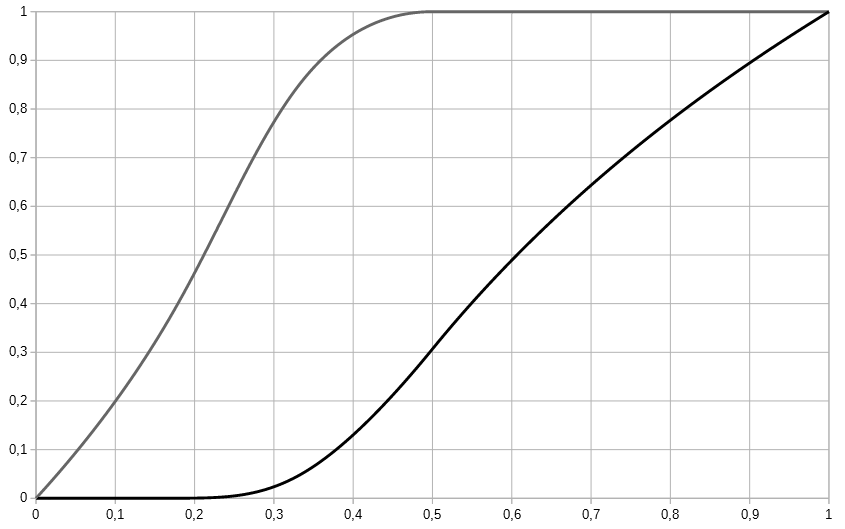
\includegraphics[width=15.5cm, angle=0]{img/F1_F2.png}
	\caption{\label{fig:F_12} $F(\alpha)$ and $F_2(\alpha)$.}
\end{figure}

The sizes of the two largest prime factors are correlated: let $n \approx 10^{100}$
and $p \approx 10^{30}$ be the largest prime factor of $n$. We have $\alpha = 0.3$
and $F(\alpha) \approx 0.02365$. However $F_2(0.0131) \approx 0.02365$ and
$n^{0.0131} \approx 20.4$.
The probability that the largest prime factor of $n$ is at most $10^{30}$ is equal to
the probability that its second largest prime factor is at most $20.4$. But this result
cannot be used to set $B_1$ and $B_2$. If the largest prime factor of $n$ is a 30-digit
prime, the second largest prime factor is certainly larger than $20.4$
(see \autoref{chap:ratio_B2_B1}).

\section{Probabilities}

Let $B_1$ and $B_2$ be the bounds of a two-stage ECM, $n$ be the number of curves and $p$
be a prime factor of $F_{12}$. $\mathcal{P}(B_1, B_2, n, p)$ is the chance for ECM to
find $p$.

If ECM finds $p$, because of Hasse's theorem we have $\#E \approx p$. $F(\alpha)$ is the probability that
the largest prime factor of $\#E$ is at most $p^\alpha$. One must have $B_2 \gtrsim p^\alpha$.
Let $P(B_2) = F(\log B_2\, /\, \log p)$. If the second largest prime factor is larger than $B_1$
then the likelihood of success for ECM is
$\mathcal{P}(B_2, B_2, n, p) = 1 - \left(1 - P(B_2) \right)^n$.

Note that $\lim\limits_{n \to \infty} \left(1 - x/n \right)^n = e^{-x}$. Hence, if
$P(B_2) \ll 1$ we have $\mathcal{P}(B_2, B_2, n, p) \approx 1 - e^{-P(B_2)\, n}$.
If $\mathcal{P}^*(B_2, B_2, n, p) = 1 - e^{-1} \approx 63.2\%$ is chosen as an acceptable
likelihood of success, we have the condition $P(B_2)\, n = 1.$

The number of operations per curve is about $\log(B_1\#) \sim B_1$ for stage 1 and about
$B_2 / \log B_2$ for stage 2 if $B_1 \ll B_2$. Hence, computation time is proportional to
$\left(B_1 + B_2 / \log B_2 \right)\, n$. If $B_1 = K \cdot B_2 / \log B_2$ then
$\left(B_2 / \log B_2 \right)\, n$ must be minimal.

Finally the conditions are $B_2$ is the maximum point of $P(B_2) \log B_2 /\, B_2$
and $n = 1 / P(B_2)$.

\begin{figure}[!h]
	\centering
	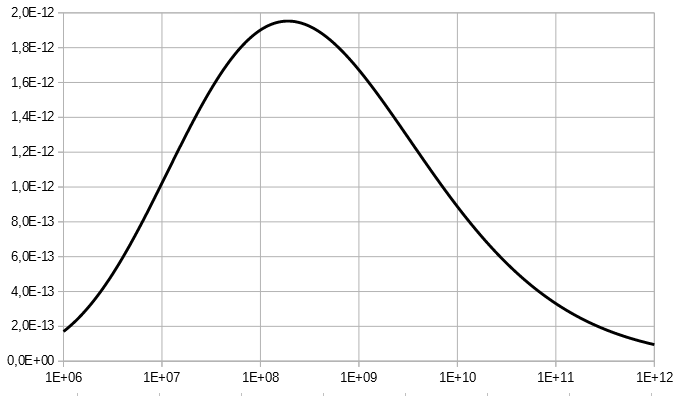
\includegraphics[width=15.5cm, angle=0]{img/cond_max.png}
	\caption{\label{fig:max} $P(B_2) \log B_2 /\, B_2$ for $p = 5\cdot10^{49}$.}
\end{figure}

Let $p = 5\cdot10^{49}$ be an average 50-digit prime.
$P(B_2) \log B_2 /\, B_2$ is maximum at $B_2 \approx 1.9\cdot 10^8$.\\
We have $P(B_2) \approx 1.95\cdot 10^{-5}$ and $n \approx 51400$.

\begin{figure}[!ht]
	\centering
	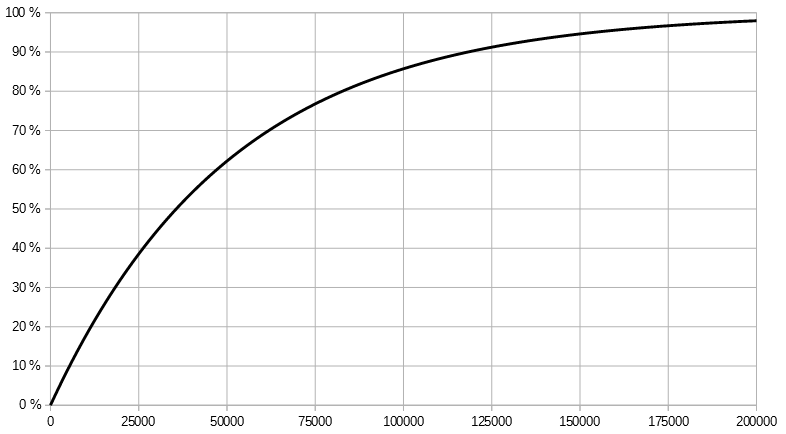
\includegraphics[width=15.5cm, angle=0]{img/n_curves.png}
	\caption{\label{fig:p_n} Probability of success for $n$ curves, $p = 5\cdot10^{49}$ and $B_2 = 1.9\cdot 10^8$.}
\end{figure}

\begin{figure}[!ht]
	\vspace*{1cm}
	\centering
	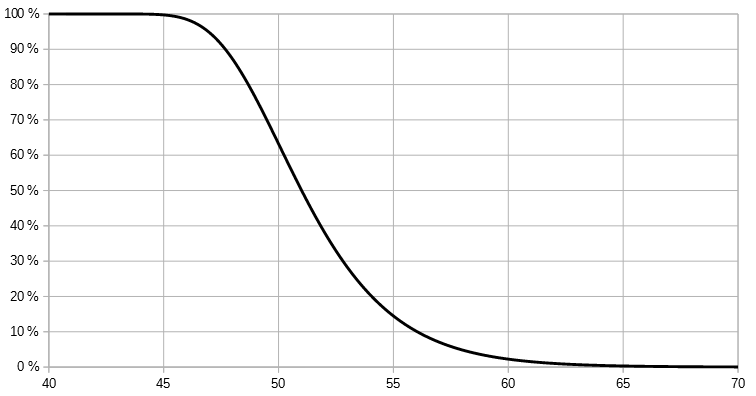
\includegraphics[width=15.5cm, angle=0]{img/prob_digits.png}
	\caption{\label{fig:p_dgt} Chance to find a $x$-digit factor, $B_2 = 190\cdot 10^6$ and $n = 51400$.}
\end{figure}

\begin{figure}[!ht]
	\vspace*{2cm}
	\centering
	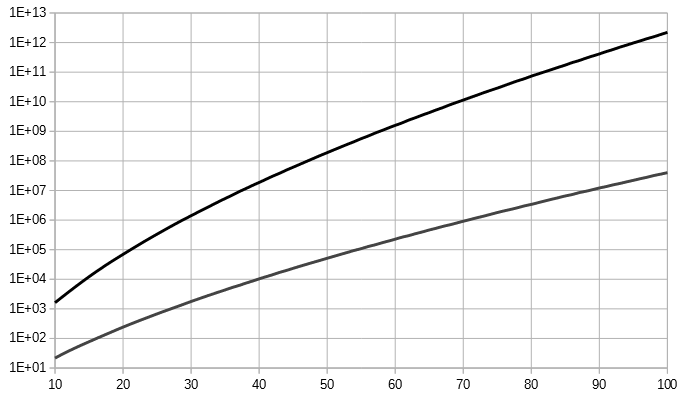
\includegraphics[width=15.5cm, angle=0]{img/B2_n_digits.png}
	\caption{\label{fig:B2_dgt} Optimal $B_2$ and number of curves as a function of the number of digits.}
\end{figure}

\subsection{The ratio $B_2 / B_1$} \label{chap:ratio_B2_B1}

The generalized Dickman function $F_2$ cannot be used to compute $B_1$ as a function of $B_2$ (see \autoref{chap:l_prm_fact}). Let $G(\alpha, \beta)$ be the probability that the largest prime factor
of a number $n$ is at most $n^\alpha$ and that the second largest prime factor of $n$ is at most
$n^\beta$. Following Knuth and Trabb Pardo \cite{KnuthPardo1} heuristic derivation, we have:
\begin{equation*}
G(\alpha, \beta) = \begin{cases}
F(\beta) + \int_\beta^\alpha F \left(\frac{\beta}{1-t} \right) \frac{dt}{t} & \text{if } 0 \leq \beta < \alpha \text{,}\\
F(\alpha) & \text{if } \beta \geq \alpha \text{.}
\end{cases}
\end{equation*}
If $\beta \leq \alpha$ we have
$G(\alpha, \beta) = F(\beta) + \int_\beta^\alpha \rho \left(\frac{1-t}{\beta} \right) \frac{dt}{t}$
and $G(1/u, 1/v) = \rho(v) + \int_{1/v}^{1/u} \rho \left((1-t)\, v \right) \frac{dt}{t}$.

Let $t' = (1-t)\, v + 1$. We have $t = (v + 1 - t')/v$, $dt = -dt'/v$ and
$\frac{dt}{t} = -\frac{dt'}{v + 1 - t'}$. Hence,
$$G(1/u, 1/v) = \sigma(u, v) = \rho(v) + \int_{v + 1 - v/u}^v \frac{\rho(t - 1)\, dt}{v + 1 - t}.$$
This relation can be used for the numerical computation of $\sigma$.

$P(B_2) = F(\log B_2\, /\, \log p)$ can be replaced with $P(B_2, B_1) = G(\log B_2\, /\, \log p,
\log B_1\, /\, \log p)$. Now the likelihood of success for ECM is
$\mathcal{P}(B_2, B_1, n, p) = 1 - \left(1 - P(B_2, B_1) \right)^n$.

The computation time is proportional to $\left(K\cdot B_1 + B_2 / \log B_2 \right)\, n$, where
$K \approx 5.6$ depends on the implementation. Hence, $(B_2; B_1)$ must be the maximum point of the
function
$$\frac{P(B_2, B_1)}{K\cdot B_1 + B_2 / \log B_2}.$$
\begin{figure}[!ht]
	\vspace*{-0.5cm}
	\centering
	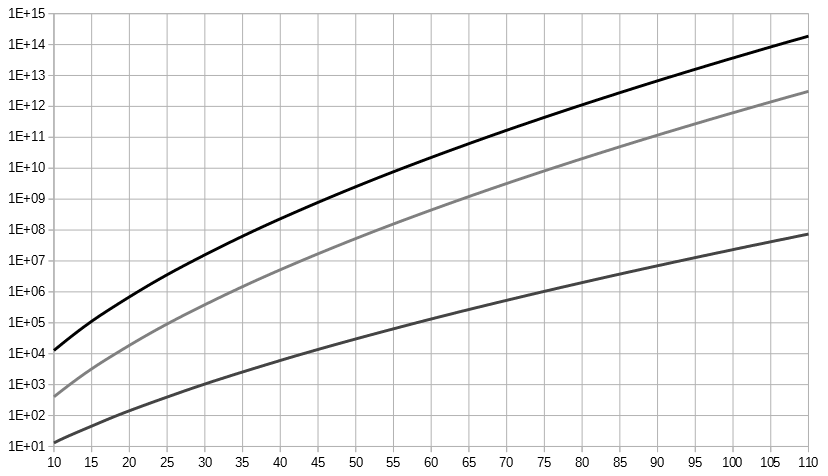
\includegraphics[width=15.5cm, angle=0]{img/B1_B2_n_digits.png}
	\caption{\label{fig:B12_dgt} Optimal $B_2, B_1$ and number of curves as a function of the number of digits.}
\end{figure}

\subsection{ECM and $F_{12}$}

The present status is
$$F_{12} = P_6 \:\cdot\: P_8 \:\cdot\: P_8 \:\cdot\: P_{12} \:\cdot\: P_{16} \:\cdot P_{54}
\:\cdot\: C_{1133}.$$
The size of the next prime factor is unknown and we can't set $B_1$ and $B_2$ as a function
of its number of digits. The number of curves needed to find a new factor is unknown but it
is a variable that will increase over time. We can set the searched prime factor as a function
of the index of the curve.

The number of digits, $B_1$ and $B_2$ can be computed as a function of number of curves
with \autoref{chap:ratio_B2_B1}. But now we don't check $n$ curves with a fixed set of
parameters but the $i^\text{th}$ curve is tested with different settings
$B_1(i)$ and $B_2(i)$.

However \autoref{chap:ratio_B2_B1} can be the starting point. For integer values of $\log p$,
$n(\lfloor\log p\rfloor)$ is calculated. If $n$ curves are tested for each value of
$\lfloor\log p\rfloor$, the probability of success is larger than $1 - e^{-1}$ because
$n(\lfloor\log p\rfloor - 1), n(\lfloor\log p\rfloor - 2), \ldots$ have already been tested.
If $n(\lfloor\log p\rfloor) - n(\lfloor\log p\rfloor - 1)$ curves are tested then
the probability is smaller than $1 - e^{-1}$ because
$B_1(\lfloor\log p\rfloor - 1) < B_1(\lfloor\log p\rfloor)$ and
$B_2(\lfloor\log p\rfloor - 1) < B_2(\lfloor\log p\rfloor)$.

We search for $\lambda$ such that if
$n'(\lfloor\log p\rfloor) = n(\lfloor\log p\rfloor) - \lambda \cdot n(\lfloor\log p\rfloor - 1)$
then the probability remains constant and equal to $1 - e^{-1}$. $\lambda \approx 0.92$ is
suitable. By inverting this function, for each index an estimate of $\log p$ is computed and
then $B_1(\log p)$ and $B_2(\log p)$.


\begin{figure}[!ht]
	\vspace*{1.0cm}
	\centering
	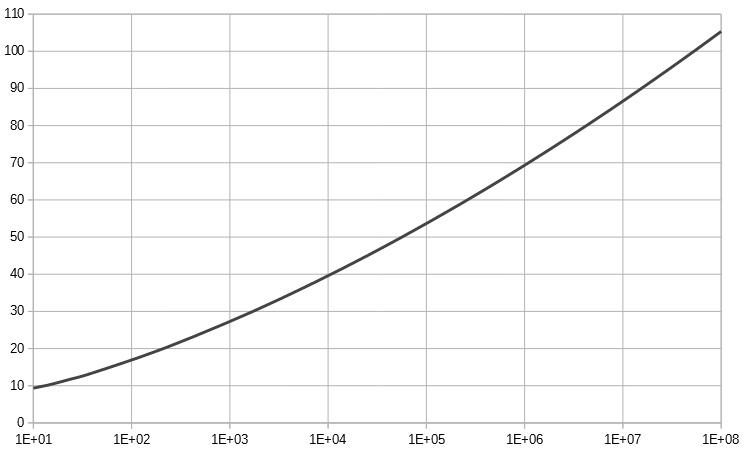
\includegraphics[width=15.5cm, angle=0]{img/digits_n.png}
	\caption{\label{fig:dgt_n} Expected number of digits as a function of the index of the curve.}
	\vspace*{1.0cm}
\end{figure}

\begin{figure}[!ht]
	\vspace*{0.0cm}
	\centering
	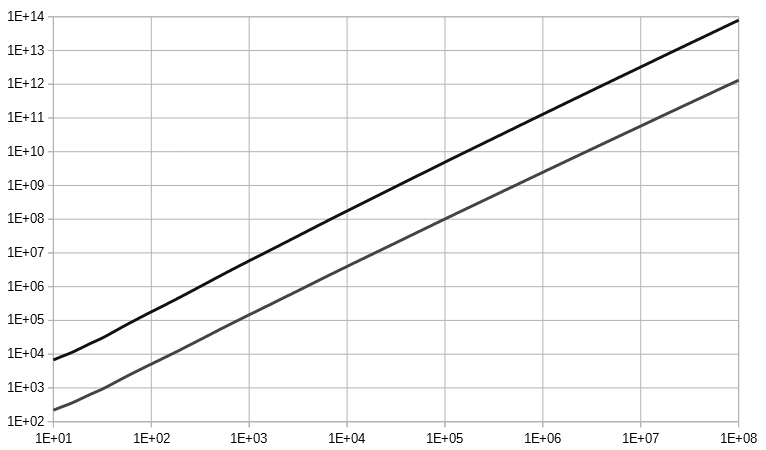
\includegraphics[width=15.5cm, angle=0]{img/B1_B2_n.png}
	\caption{\label{fig:B_12_n} $B_2$ and $B_1$ as a function of the index of the curve.}
\end{figure}

$\log B_2 = f(\log i)$ where $i$ is the $i^\text{th}$ curve is close to a linear function.
The error of the estimate $B_2 = 400\, i^{\sqrt{2}}$ is less than $5\%$ for
$10^4 \leq i \leq 10^8$. The ratio of $B_2\, /\, B_1 = 26 + 1.8\, \log{i}$ is always
slightly larger than the optimal value. Finally we have
$\log p \approx (3 + 1.3\, \log i)^{5/3}$.

The following parameters are applied: let $i$ be the $i^\text{th}$ curve and $d$ be the
expected number of digits of the prime factor, then
\begin{align*}
B_2 &= 400\, i^{\sqrt{2}},\\
B_1 &= B_2\, /\, (26 + 1.8\, \log{i}),\\
d &= (1.8 + 0.79\, \log i)^{5/3}.
\end{align*}
\begin{figure}[!ht]
	\vspace*{-0.8cm}
	\centering
	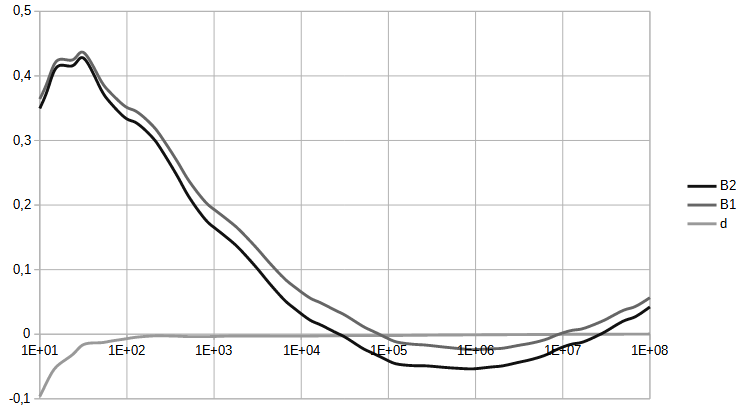
\includegraphics[width=12.0cm, angle=0]{img/err_B1_B2_digits.png}
	\caption{\label{fig:B12_n} Relative error with applied parameters as a function of the index of the curve.}
\end{figure}

\subsection{Test of the probabilistic model}



\chapter{Implementation}

\begin{thebibliography}{99}

\bibitem{BachShallit1} Eric~Bach and Jeffrey~Shallit, \emph{Factoring with cyclotomic polynomials},
Math. Comp. \textbf{52} (1989), 201--219, DOI: \url{https://doi.org/10.1090/S0025-5718-1989-0947467-1}.

\bibitem{Brent1} Richard~P.~Brent, \emph{Factorization of the tenth Fermat number}, Math. Comp.
\textbf{68} (1999), 429--451, DOI: \url{https://doi.org/10.1090/S0025-5718-99-00992-8}.

\bibitem{Brent2} Richard~P.~Brent, \emph{Factorization of the tenth and eleventh Fermat numbers},
Report TR-CS-96-02, Computer Sciences Laboratory, Australian National Univ., Canberra, Feb. 1996,
\url{https://citeseerx.ist.psu.edu/viewdoc/download?doi=10.1.1.70.6415&rep=rep1&type=pdf}.

\bibitem{BrentPollard1} Richard~P.~Brent and John~M.~Pollard, \emph{Factorization of the eighth
Fermat number}, Math. Comp. \textbf{36} (1981), 627--630, DOI:
\url{https://doi.org/10.1090/S0025-5718-1981-0606520-5}.

\bibitem{Dickman1} Karl~Dickman, \emph{On the Frequency of Numbers Containing Prime Factors
of a Certain Relative Magnitude}, Arkiv för Mat., Astron. och Fys. 22A, 1-14, 1930. 

\bibitem{Fermat1} Pierre~de~Fermat, \emph{Lettre à Marin Mersenne},
\url{https://www.archive.org/stream/oeuvresdefermat942ferm#page/212/mode/2up}.

\bibitem{Knapp1} Anthony~W.~Knapp, \emph{Elliptic Curves}, Princeton University Press,
Princeton, NJ, 1992.

\bibitem{KnuthPardo1} Donald~E.~Knuth and Luis~Trabb~Pardo, \emph{Analysis of a simple
factorization algorithm}, Theoretical Computer Science, Volume 3, Issue 3, December 1976,
Pages 321--348, DOI: \url{https://doi.org/10.1016/0304-3975(76)90050-5}.

\bibitem{Lenstra2ManassePollard} A.~K.~Lenstra, H.~W.~Lenstra, M.~S.~Manasse and J.~M.~Pollard
\emph{The factorization of the ninth Fermat number}, Math. Comp. \textbf{61} (1993), 319--349,
DOI: \url{https://doi.org/10.1090/S0025-5718-1993-1182953-4}.

\bibitem{LuneWattel1} J.~van~de~Lune and E.~Wattel, \emph{On the numerical solution of a
differential-difference equation arising in analytic number theory}, Math. Comp. \textbf{23}
(1969), 417--421, DOI: \url{https://doi.org/10.1090/S0025-5718-1969-0247789-3}.

\bibitem{MorrisonBrillhart1} Michael~A.~Morrison and John~Brillhart, \emph{A method of factoring
and the factorization of $F_7$}, Math. Comp. \textbf{29} (1975), 183--205,
DOI: \url{https://doi.org/10.1090/S0025-5718-1975-0371800-5}.

\bibitem{Pollard1} J.~M.~Pollard, \emph{Theorems on factorization and  primality testing},
Mathematical Proceedings of the Cambridge Philosophical Society, Volume \textbf{76}, Issue 3,
November 1974, pp. 521 - 528, DOI: \url{https://doi.org/10.1017/S0305004100049252}.

\bibitem{Vang1} \url{https://caramel.loria.fr/f12.txt}.

\end{thebibliography}

\end{document} 
